% Generated by Sphinx.
\def\sphinxdocclass{report}
\documentclass[letterpaper,10pt,english]{sphinxmanual}
\usepackage[utf8]{inputenc}
\DeclareUnicodeCharacter{00A0}{\nobreakspace}
\usepackage{cmap}
\usepackage[T1]{fontenc}
\usepackage{babel}
\usepackage{times}
\usepackage[Bjarne]{fncychap}
\usepackage{longtable}
\usepackage{sphinx}
\usepackage{multirow}


\title{Symtyper Documentation}
\date{August 13, 2014}
\release{0.1}
\author{}
\newcommand{\sphinxlogo}{}
\renewcommand{\releasename}{Release}
\makeindex

\makeatletter
\def\PYG@reset{\let\PYG@it=\relax \let\PYG@bf=\relax%
    \let\PYG@ul=\relax \let\PYG@tc=\relax%
    \let\PYG@bc=\relax \let\PYG@ff=\relax}
\def\PYG@tok#1{\csname PYG@tok@#1\endcsname}
\def\PYG@toks#1+{\ifx\relax#1\empty\else%
    \PYG@tok{#1}\expandafter\PYG@toks\fi}
\def\PYG@do#1{\PYG@bc{\PYG@tc{\PYG@ul{%
    \PYG@it{\PYG@bf{\PYG@ff{#1}}}}}}}
\def\PYG#1#2{\PYG@reset\PYG@toks#1+\relax+\PYG@do{#2}}

\expandafter\def\csname PYG@tok@gd\endcsname{\def\PYG@tc##1{\textcolor[rgb]{0.63,0.00,0.00}{##1}}}
\expandafter\def\csname PYG@tok@gu\endcsname{\let\PYG@bf=\textbf\def\PYG@tc##1{\textcolor[rgb]{0.50,0.00,0.50}{##1}}}
\expandafter\def\csname PYG@tok@gt\endcsname{\def\PYG@tc##1{\textcolor[rgb]{0.00,0.27,0.87}{##1}}}
\expandafter\def\csname PYG@tok@gs\endcsname{\let\PYG@bf=\textbf}
\expandafter\def\csname PYG@tok@gr\endcsname{\def\PYG@tc##1{\textcolor[rgb]{1.00,0.00,0.00}{##1}}}
\expandafter\def\csname PYG@tok@cm\endcsname{\let\PYG@it=\textit\def\PYG@tc##1{\textcolor[rgb]{0.25,0.50,0.56}{##1}}}
\expandafter\def\csname PYG@tok@vg\endcsname{\def\PYG@tc##1{\textcolor[rgb]{0.73,0.38,0.84}{##1}}}
\expandafter\def\csname PYG@tok@m\endcsname{\def\PYG@tc##1{\textcolor[rgb]{0.13,0.50,0.31}{##1}}}
\expandafter\def\csname PYG@tok@mh\endcsname{\def\PYG@tc##1{\textcolor[rgb]{0.13,0.50,0.31}{##1}}}
\expandafter\def\csname PYG@tok@cs\endcsname{\def\PYG@tc##1{\textcolor[rgb]{0.25,0.50,0.56}{##1}}\def\PYG@bc##1{\setlength{\fboxsep}{0pt}\colorbox[rgb]{1.00,0.94,0.94}{\strut ##1}}}
\expandafter\def\csname PYG@tok@ge\endcsname{\let\PYG@it=\textit}
\expandafter\def\csname PYG@tok@vc\endcsname{\def\PYG@tc##1{\textcolor[rgb]{0.73,0.38,0.84}{##1}}}
\expandafter\def\csname PYG@tok@il\endcsname{\def\PYG@tc##1{\textcolor[rgb]{0.13,0.50,0.31}{##1}}}
\expandafter\def\csname PYG@tok@go\endcsname{\def\PYG@tc##1{\textcolor[rgb]{0.20,0.20,0.20}{##1}}}
\expandafter\def\csname PYG@tok@cp\endcsname{\def\PYG@tc##1{\textcolor[rgb]{0.00,0.44,0.13}{##1}}}
\expandafter\def\csname PYG@tok@gi\endcsname{\def\PYG@tc##1{\textcolor[rgb]{0.00,0.63,0.00}{##1}}}
\expandafter\def\csname PYG@tok@gh\endcsname{\let\PYG@bf=\textbf\def\PYG@tc##1{\textcolor[rgb]{0.00,0.00,0.50}{##1}}}
\expandafter\def\csname PYG@tok@ni\endcsname{\let\PYG@bf=\textbf\def\PYG@tc##1{\textcolor[rgb]{0.84,0.33,0.22}{##1}}}
\expandafter\def\csname PYG@tok@nl\endcsname{\let\PYG@bf=\textbf\def\PYG@tc##1{\textcolor[rgb]{0.00,0.13,0.44}{##1}}}
\expandafter\def\csname PYG@tok@nn\endcsname{\let\PYG@bf=\textbf\def\PYG@tc##1{\textcolor[rgb]{0.05,0.52,0.71}{##1}}}
\expandafter\def\csname PYG@tok@no\endcsname{\def\PYG@tc##1{\textcolor[rgb]{0.38,0.68,0.84}{##1}}}
\expandafter\def\csname PYG@tok@na\endcsname{\def\PYG@tc##1{\textcolor[rgb]{0.25,0.44,0.63}{##1}}}
\expandafter\def\csname PYG@tok@nb\endcsname{\def\PYG@tc##1{\textcolor[rgb]{0.00,0.44,0.13}{##1}}}
\expandafter\def\csname PYG@tok@nc\endcsname{\let\PYG@bf=\textbf\def\PYG@tc##1{\textcolor[rgb]{0.05,0.52,0.71}{##1}}}
\expandafter\def\csname PYG@tok@nd\endcsname{\let\PYG@bf=\textbf\def\PYG@tc##1{\textcolor[rgb]{0.33,0.33,0.33}{##1}}}
\expandafter\def\csname PYG@tok@ne\endcsname{\def\PYG@tc##1{\textcolor[rgb]{0.00,0.44,0.13}{##1}}}
\expandafter\def\csname PYG@tok@nf\endcsname{\def\PYG@tc##1{\textcolor[rgb]{0.02,0.16,0.49}{##1}}}
\expandafter\def\csname PYG@tok@si\endcsname{\let\PYG@it=\textit\def\PYG@tc##1{\textcolor[rgb]{0.44,0.63,0.82}{##1}}}
\expandafter\def\csname PYG@tok@s2\endcsname{\def\PYG@tc##1{\textcolor[rgb]{0.25,0.44,0.63}{##1}}}
\expandafter\def\csname PYG@tok@vi\endcsname{\def\PYG@tc##1{\textcolor[rgb]{0.73,0.38,0.84}{##1}}}
\expandafter\def\csname PYG@tok@nt\endcsname{\let\PYG@bf=\textbf\def\PYG@tc##1{\textcolor[rgb]{0.02,0.16,0.45}{##1}}}
\expandafter\def\csname PYG@tok@nv\endcsname{\def\PYG@tc##1{\textcolor[rgb]{0.73,0.38,0.84}{##1}}}
\expandafter\def\csname PYG@tok@s1\endcsname{\def\PYG@tc##1{\textcolor[rgb]{0.25,0.44,0.63}{##1}}}
\expandafter\def\csname PYG@tok@gp\endcsname{\let\PYG@bf=\textbf\def\PYG@tc##1{\textcolor[rgb]{0.78,0.36,0.04}{##1}}}
\expandafter\def\csname PYG@tok@sh\endcsname{\def\PYG@tc##1{\textcolor[rgb]{0.25,0.44,0.63}{##1}}}
\expandafter\def\csname PYG@tok@ow\endcsname{\let\PYG@bf=\textbf\def\PYG@tc##1{\textcolor[rgb]{0.00,0.44,0.13}{##1}}}
\expandafter\def\csname PYG@tok@sx\endcsname{\def\PYG@tc##1{\textcolor[rgb]{0.78,0.36,0.04}{##1}}}
\expandafter\def\csname PYG@tok@bp\endcsname{\def\PYG@tc##1{\textcolor[rgb]{0.00,0.44,0.13}{##1}}}
\expandafter\def\csname PYG@tok@c1\endcsname{\let\PYG@it=\textit\def\PYG@tc##1{\textcolor[rgb]{0.25,0.50,0.56}{##1}}}
\expandafter\def\csname PYG@tok@kc\endcsname{\let\PYG@bf=\textbf\def\PYG@tc##1{\textcolor[rgb]{0.00,0.44,0.13}{##1}}}
\expandafter\def\csname PYG@tok@c\endcsname{\let\PYG@it=\textit\def\PYG@tc##1{\textcolor[rgb]{0.25,0.50,0.56}{##1}}}
\expandafter\def\csname PYG@tok@mf\endcsname{\def\PYG@tc##1{\textcolor[rgb]{0.13,0.50,0.31}{##1}}}
\expandafter\def\csname PYG@tok@err\endcsname{\def\PYG@bc##1{\setlength{\fboxsep}{0pt}\fcolorbox[rgb]{1.00,0.00,0.00}{1,1,1}{\strut ##1}}}
\expandafter\def\csname PYG@tok@kd\endcsname{\let\PYG@bf=\textbf\def\PYG@tc##1{\textcolor[rgb]{0.00,0.44,0.13}{##1}}}
\expandafter\def\csname PYG@tok@ss\endcsname{\def\PYG@tc##1{\textcolor[rgb]{0.32,0.47,0.09}{##1}}}
\expandafter\def\csname PYG@tok@sr\endcsname{\def\PYG@tc##1{\textcolor[rgb]{0.14,0.33,0.53}{##1}}}
\expandafter\def\csname PYG@tok@mo\endcsname{\def\PYG@tc##1{\textcolor[rgb]{0.13,0.50,0.31}{##1}}}
\expandafter\def\csname PYG@tok@mi\endcsname{\def\PYG@tc##1{\textcolor[rgb]{0.13,0.50,0.31}{##1}}}
\expandafter\def\csname PYG@tok@kn\endcsname{\let\PYG@bf=\textbf\def\PYG@tc##1{\textcolor[rgb]{0.00,0.44,0.13}{##1}}}
\expandafter\def\csname PYG@tok@o\endcsname{\def\PYG@tc##1{\textcolor[rgb]{0.40,0.40,0.40}{##1}}}
\expandafter\def\csname PYG@tok@kr\endcsname{\let\PYG@bf=\textbf\def\PYG@tc##1{\textcolor[rgb]{0.00,0.44,0.13}{##1}}}
\expandafter\def\csname PYG@tok@s\endcsname{\def\PYG@tc##1{\textcolor[rgb]{0.25,0.44,0.63}{##1}}}
\expandafter\def\csname PYG@tok@kp\endcsname{\def\PYG@tc##1{\textcolor[rgb]{0.00,0.44,0.13}{##1}}}
\expandafter\def\csname PYG@tok@w\endcsname{\def\PYG@tc##1{\textcolor[rgb]{0.73,0.73,0.73}{##1}}}
\expandafter\def\csname PYG@tok@kt\endcsname{\def\PYG@tc##1{\textcolor[rgb]{0.56,0.13,0.00}{##1}}}
\expandafter\def\csname PYG@tok@sc\endcsname{\def\PYG@tc##1{\textcolor[rgb]{0.25,0.44,0.63}{##1}}}
\expandafter\def\csname PYG@tok@sb\endcsname{\def\PYG@tc##1{\textcolor[rgb]{0.25,0.44,0.63}{##1}}}
\expandafter\def\csname PYG@tok@k\endcsname{\let\PYG@bf=\textbf\def\PYG@tc##1{\textcolor[rgb]{0.00,0.44,0.13}{##1}}}
\expandafter\def\csname PYG@tok@se\endcsname{\let\PYG@bf=\textbf\def\PYG@tc##1{\textcolor[rgb]{0.25,0.44,0.63}{##1}}}
\expandafter\def\csname PYG@tok@sd\endcsname{\let\PYG@it=\textit\def\PYG@tc##1{\textcolor[rgb]{0.25,0.44,0.63}{##1}}}

\def\PYGZbs{\char`\\}
\def\PYGZus{\char`\_}
\def\PYGZob{\char`\{}
\def\PYGZcb{\char`\}}
\def\PYGZca{\char`\^}
\def\PYGZam{\char`\&}
\def\PYGZlt{\char`\<}
\def\PYGZgt{\char`\>}
\def\PYGZsh{\char`\#}
\def\PYGZpc{\char`\%}
\def\PYGZdl{\char`\$}
\def\PYGZhy{\char`\-}
\def\PYGZsq{\char`\'}
\def\PYGZdq{\char`\"}
\def\PYGZti{\char`\~}
% for compatibility with earlier versions
\def\PYGZat{@}
\def\PYGZlb{[}
\def\PYGZrb{]}
\makeatother

\begin{document}

\maketitle
\tableofcontents
\phantomsection\label{index::doc}


Contents:


\chapter{Web-based SymTyper}
\label{Web::doc}\label{Web:welcome-to-symtyper-s-documentation}\label{Web:web-based-symtyper}

\section{Brief Overview}
\label{Web:brief-overview}
To run SymTyper from the web, follow these instructions:

First, invoke symtyper main submission page (\href{http://www.symtyper.com}{http://www.symtyper.com}). You should be presented with the following page in {\hyperref[Web:fig1]{\emph{SymTyper's Main Screen}}}.
\begin{figure}[htbp]
\centering
\capstart

\scalebox{0.500000}{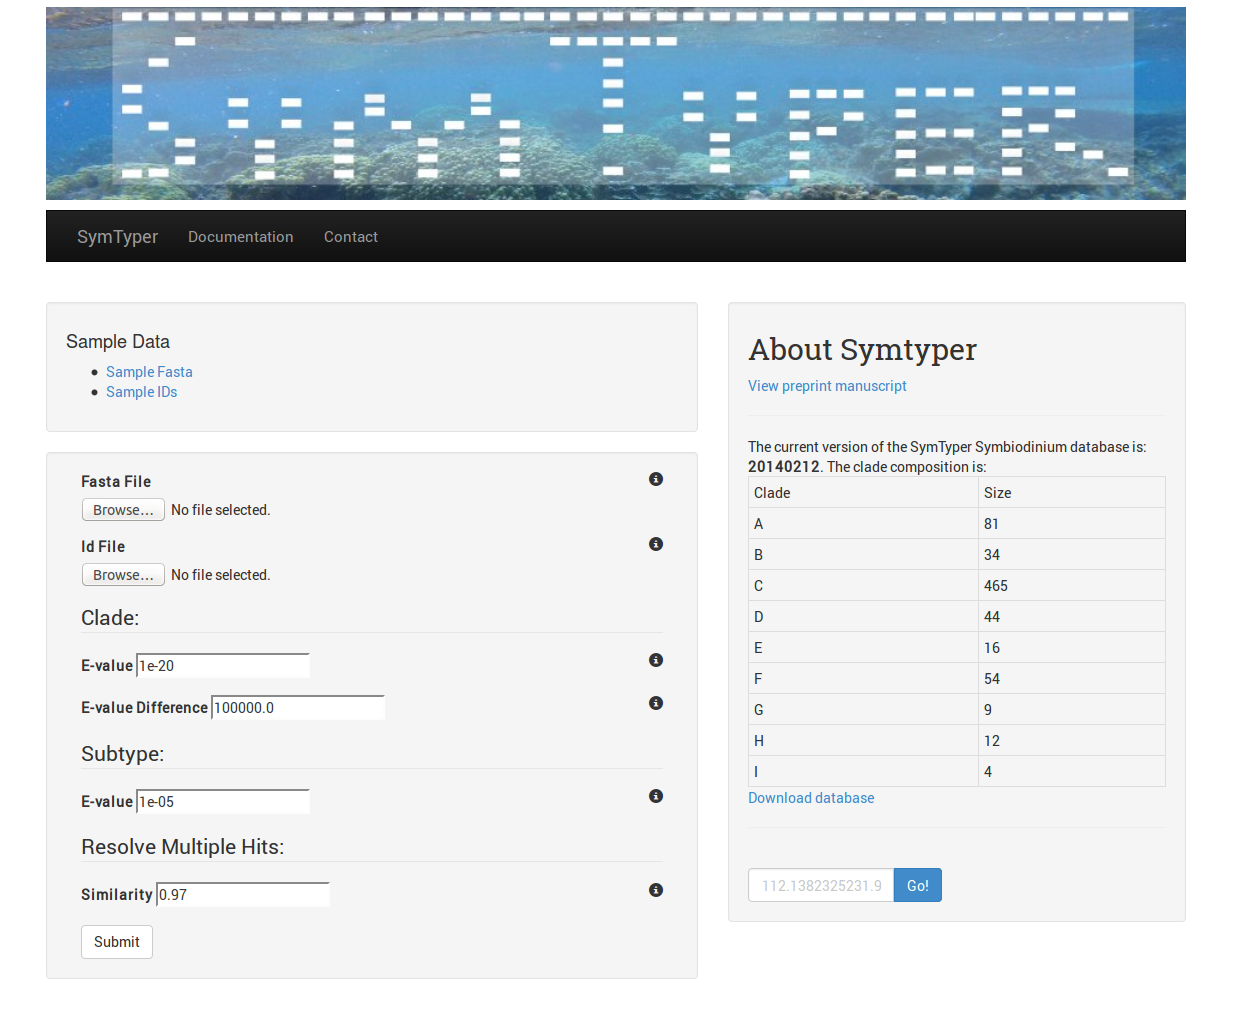
\includegraphics{main.png}}
\caption{SymTyper's Main Screen}\label{Web:fig1}\end{figure}

To submit a new analysis, browse and select your input fasta file and a valid  ids file ({\hyperref[defs:inputformat]{\emph{Fasta Input Format}}}) and then click submit.
\begin{figure}[htbp]
\centering
\capstart

\scalebox{0.500000}{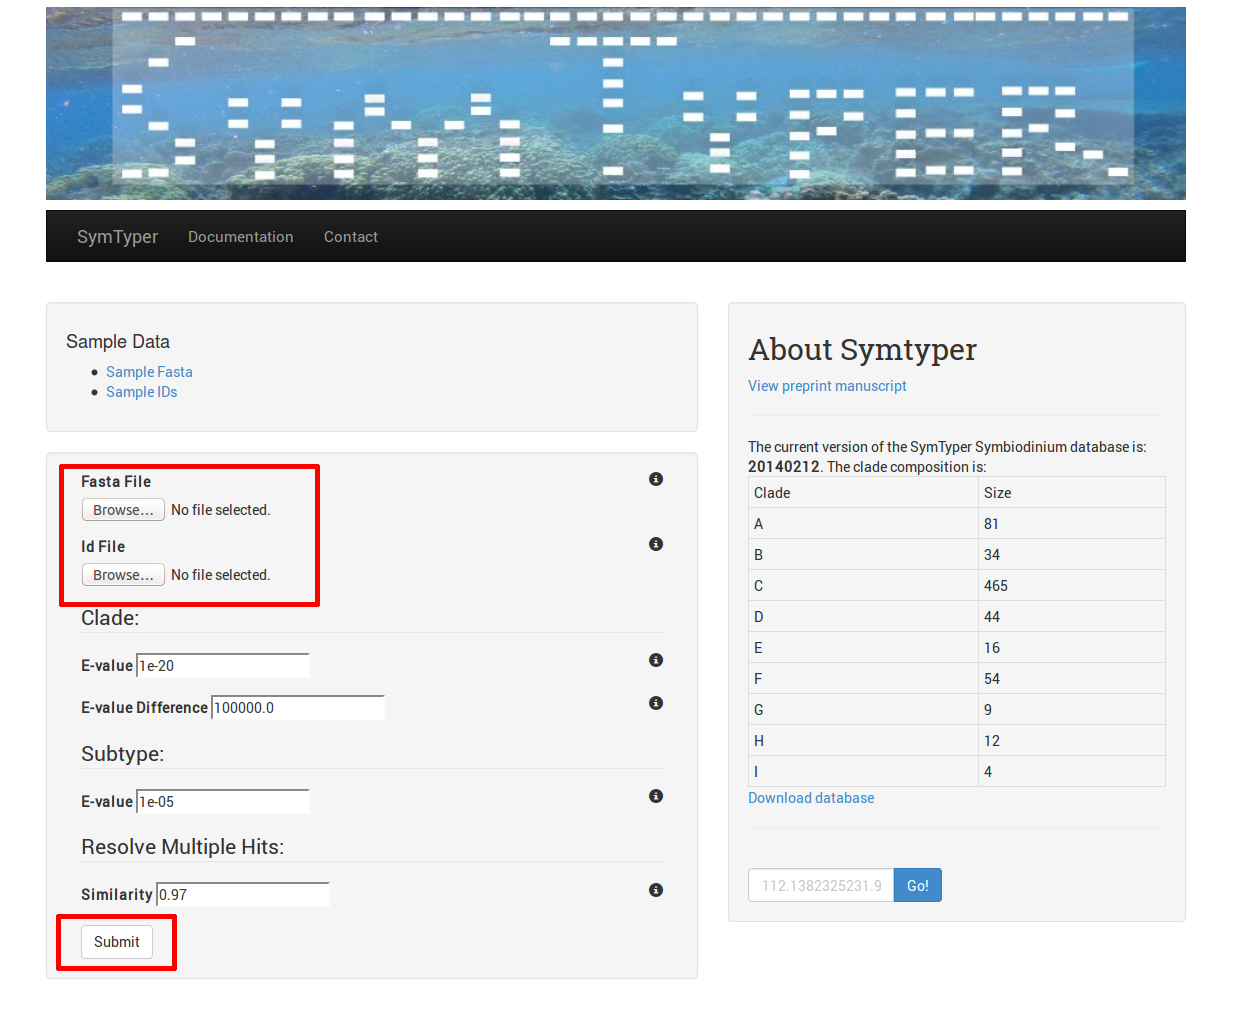
\includegraphics{submit_input.png}}
\caption{Submitting a New SymTyper Analysis}\end{figure}

The next screen will provide you with the URL where the output can be accessed.
Depending on the input size, the processing can take between few minutes to hours.
Please copy the URL for future access. Job will be hosted on the SymTyper site for 15 days.
\begin{figure}[htbp]
\centering
\capstart

\scalebox{0.500000}{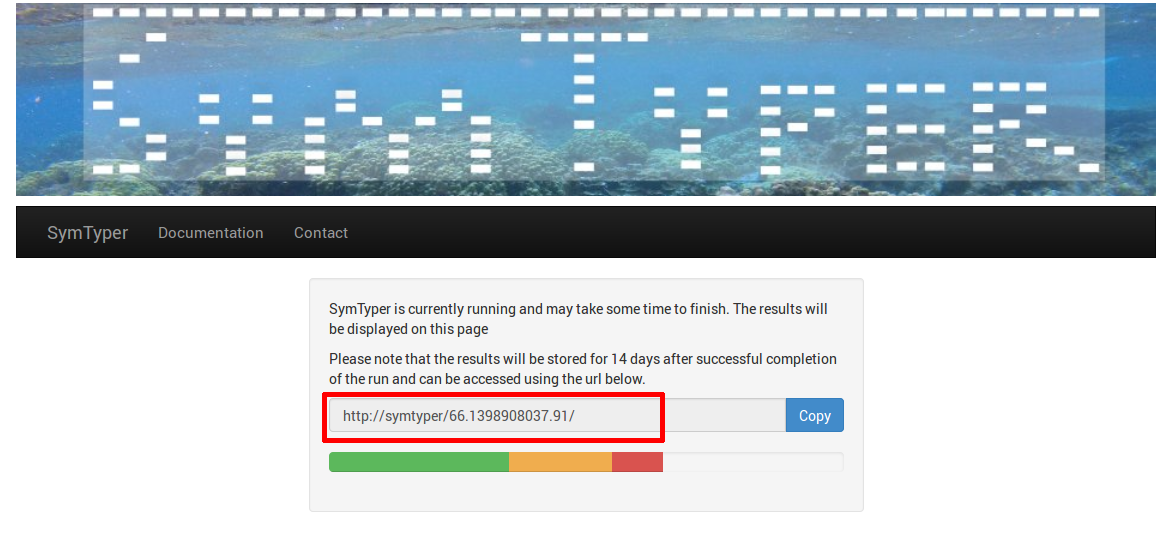
\includegraphics{processing.png}}
\caption{Processing Screen and Job URL}\end{figure}

If the anlysis completed successfully, you will be presented with
the a summary table where the various componenents of the analysis
can be accessed. The results are gouped by section: Clades, Subtypes, Multiples, Trees, Breakdown. These sections are explained below.
\begin{figure}[htbp]
\centering
\capstart

\scalebox{0.500000}{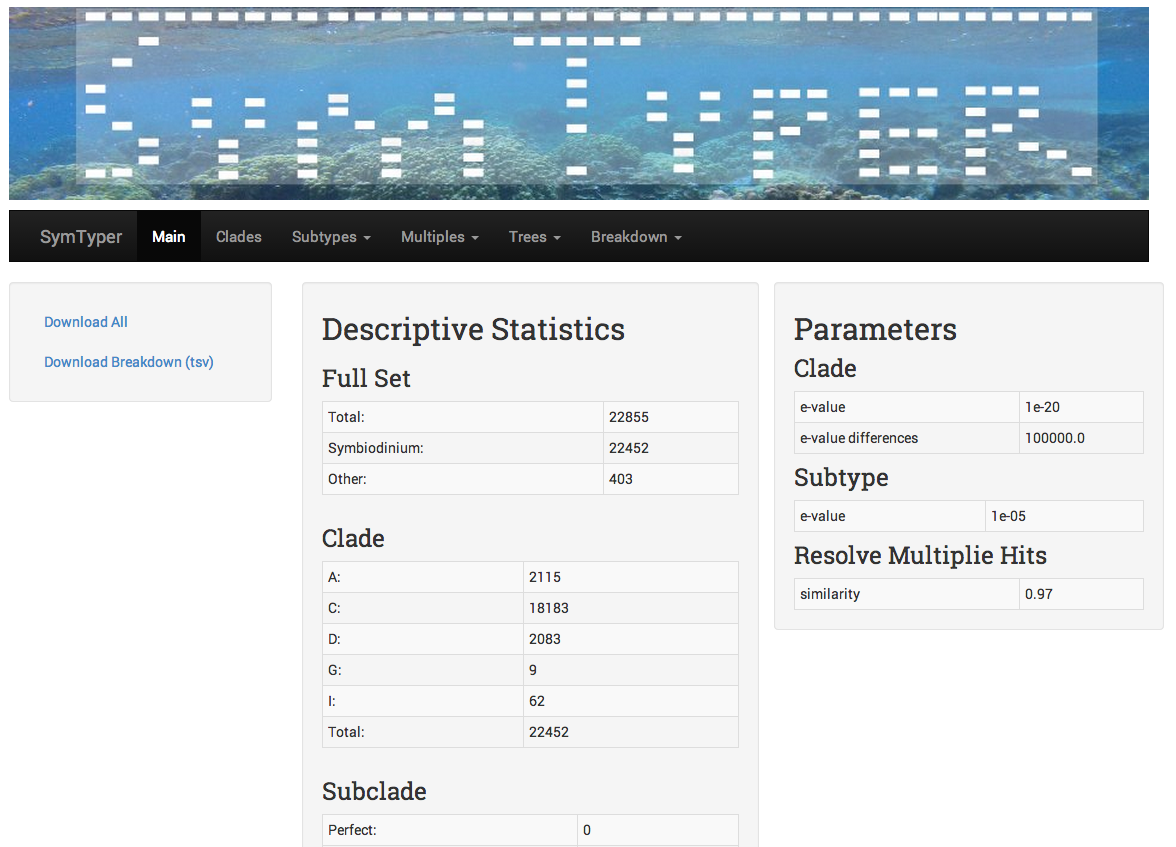
\includegraphics{results.png}}
\caption{SymTyper Results Main Screen}\label{Web:main-results-page}\end{figure}

\begin{tabulary}{\linewidth}{|p{2cm}|p{13cm}|}
\hline
\textsf{\relax 
Section
} & \textsf{\relax 
Description
}\\
\hline
Clades
 & 
Shows the breakdown of clades per sample. The results can be viewed or download as a matrix or show as a piechart per sample
\\

Subtypes
 & 
Shows the breakdowns of subtypes per sample. The results can be viewed independently for the {\hyperref[defs:perfect]{\emph{Perfect}}}, {\hyperref[defs:unique]{\emph{Unique}}} and  {\hyperref[defs:shortnew]{\emph{ShortNew}}} subtypes
\\

Multiples
 & 
The graphs shows the distribution of sequences for each clade contaning multiple hits. The definition of a Multiple hits is described in the {\hyperref[defs:multiples]{\emph{Multiples}}} section
\\

Trees
 & 
Describes the breakdown of the number of sequences assigned to the internal nodes, and the clades per sample. The tree representation show the combined count for all the samples
\\

Breakdown
 & 
Shows a Sunburst representation of the Clades and subtypes by sample
\\
\hline\end{tabulary}



\subsection{Clades View}
\label{Web:clades-view}
The Clades View shows a table view of the distribution of HITS,
NOHITS, LOW and AMBIGUOUS hits per sample.  Clicking the View Chart
provides access to the clades distribution for each sample. The
complete results and disbtribution of clades per sample can be
downloaded from the results main page (see {\hyperref[Web:main-results-page]{\emph{SymTyper Results Main Screen}}}).
\begin{figure}[htbp]
\centering
\capstart

\scalebox{0.500000}{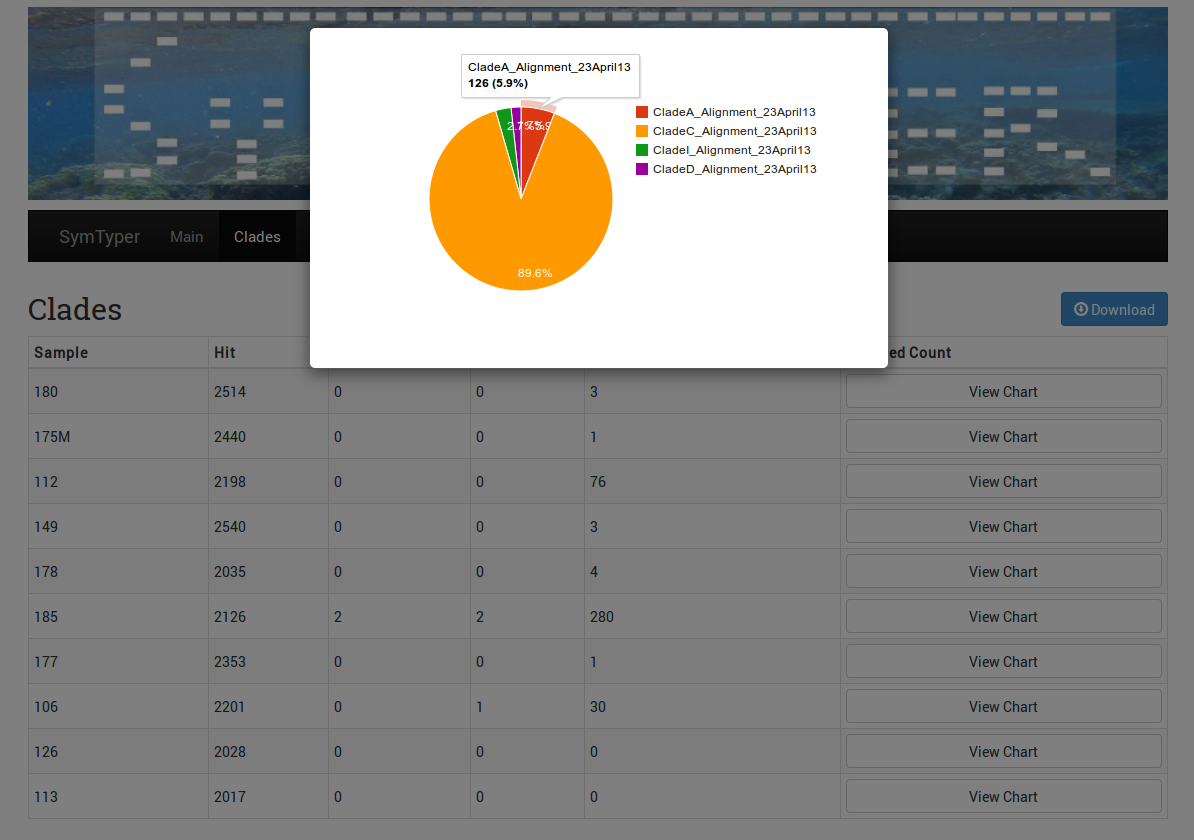
\includegraphics{pie_chart.png}}
\caption{Pie Chart Distribution of Clade per Sample}\end{figure}


\subsection{Subtypes View}
\label{Web:subtypes-view}
The Subtypes Views shows the breakdown of subtypes per sample. The results
can be viewed independently for the {\hyperref[defs:perfect]{\emph{Perfect}}}, {\hyperref[defs:unique]{\emph{Unique}}} and the
{\hyperref[defs:shortnew]{\emph{ShortNew}}} subtypes. The subtypes are assigned based on the blast results of the query sequences to
the clade specific references.
\begin{figure}[htbp]
\centering
\capstart

\scalebox{0.600000}{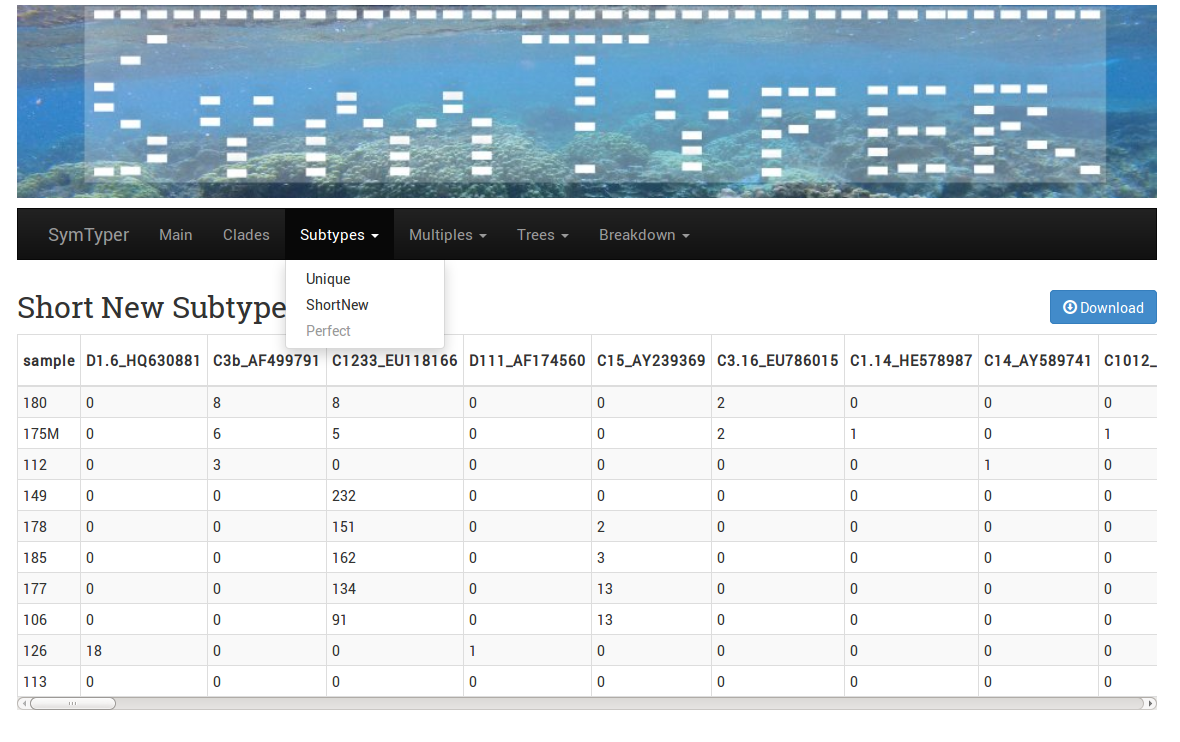
\includegraphics{subtypes.png}}
\caption{Subtypes Distribution per Clade}\end{figure}

\begin{tabulary}{\linewidth}{|p{2cm}|p{13cm}|}
\hline
\textsf{\relax 
Section
} & \textsf{\relax 
Description
}\\
\hline
Perfect
 & 
A query sequence that aligns perfectly or with very high similarity to a unique symbiont reference in the database (e.g., 100\% similarity to 100\% of the length of the target)
\\

Unique
 & 
A query sequence that aligns unambiguously to symbiont reference in the database. (e.g., \(>=\) user defined \% similarity to 100\% target length and the bit score for the best hit is at least 3 orders or magnitude larger than than that for the second hit);
\\

ShortNew
 & 
A query sequence shorter than the average sequence in the reference database but aligns with high similarity to a unique reference according to the dynamic similarity threshold (See {\hyperref[defs:dynamic-similarity]{\emph{Dynamic Similarity}}})
\\
\hline\end{tabulary}



\subsection{Multiples View}
\label{Web:multiples-view}
The Multiples View is a graphical representation of the corrected subtypes
count to which ambiguous sequences map. The algortihm used to
resolved multiple hits is described in the {\hyperref[defs:multiple-hits]{\emph{Ambiguous Hit Correction}}} and
detailed in the manuscript.
\begin{figure}[htbp]
\centering
\capstart

\scalebox{0.500000}{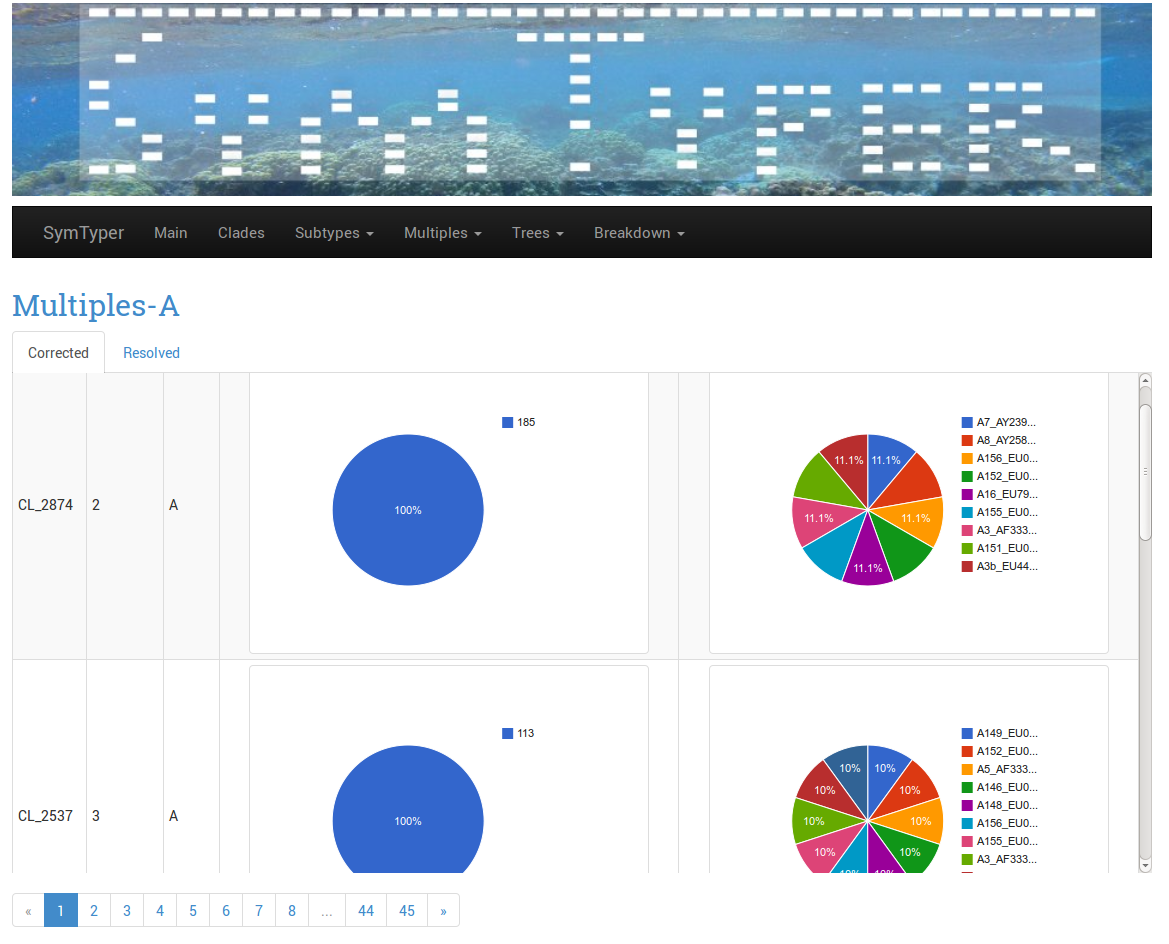
\includegraphics{multiples.png}}
\caption{Subtypes Distribution for the Corrected Ambiguous Hits}\end{figure}

The breakedown of subtypes for {\hyperref[defs:resolved]{\emph{Resolved}}} under the ``Resolved tab''


\subsection{Trees View}
\label{Web:trees-view}\begin{figure}[htbp]
\centering
\capstart

\scalebox{0.500000}{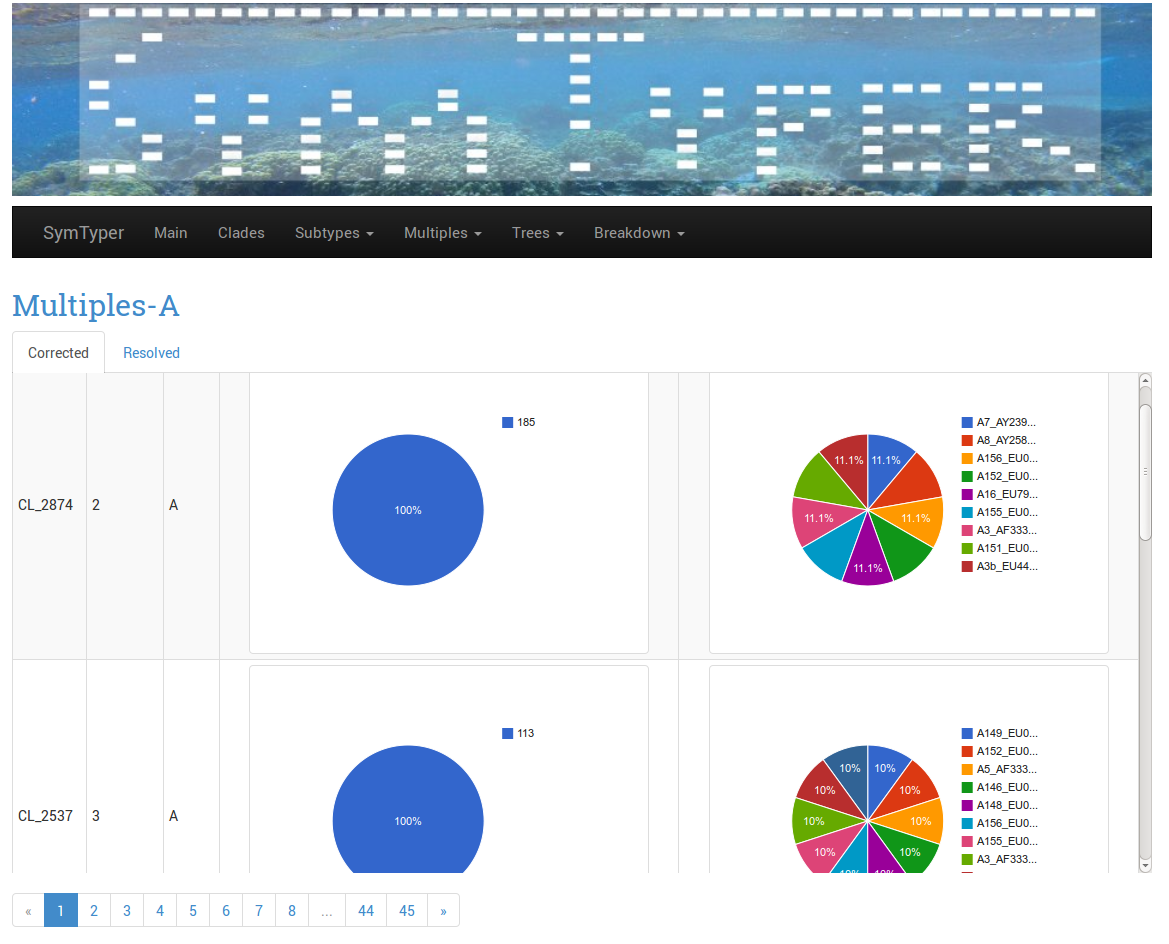
\includegraphics{multiples.png}}
\caption{Distribution of Ambiguous Sequences in the Clade Phylogeny.}\end{figure}

For each clade phylogeny, this view compiles the number of times a {\hyperref[defs:lca]{\emph{Lowest Common Ancestor}}}
was identified for an ambiguous sequence (after the {\hyperref[defs:multiple-hits]{\emph{Ambiguous Hit Correction}}} stage).
The tree can be downloaded in the Newick format and viewed or parsed in phylogeny
applications. A matrix file comparing results across samples can be be found in
output archive available for download from the main page.


\subsection{Breakdown View}
\label{Web:breakdown-view}\begin{figure}[htbp]
\centering

\scalebox{0.500000}{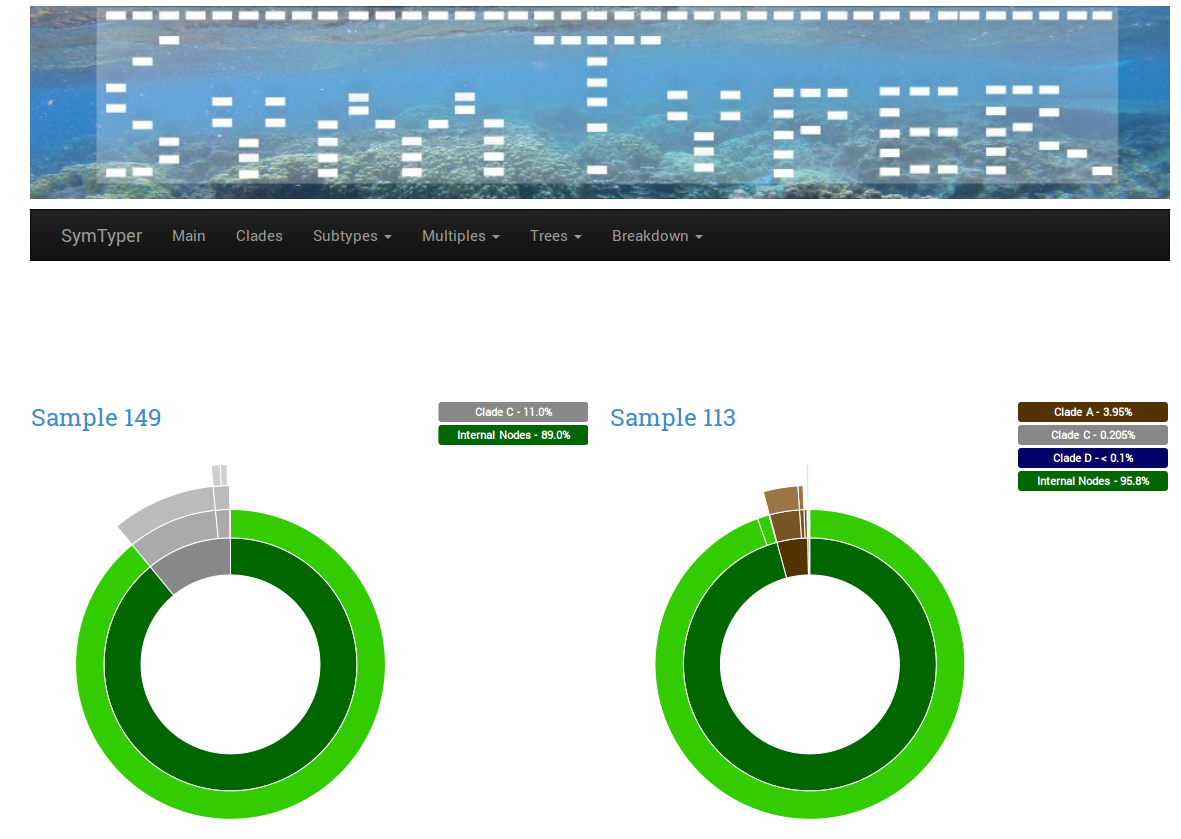
\includegraphics{breakdown.png}}
\end{figure}

Using user-friendly graphical Sunburst representation,
this view summarizes the intricate structure of Symbiodinium clades and subtypes
in a single or multi-sample view. Highlighting a level of the Sunburst charts display
its structure and the percentage of sample reads assigned to it.


\chapter{Command Line Symtyper}
\label{CommandLine::doc}\label{CommandLine:command-line-symtyper}

\section{Installing Symtyper's requirements}
\label{CommandLine:installing-symtyper-s-requirements}
The most recent version of Symtyper is a self-contained Python script that can be run without being explicitly installed on the system.
However, Symtyper depends on other applciation for its exectution. These applications are

\begin{tabulary}{\linewidth}{|L|L|L|}
\hline
\textsf{\relax 
Application
} & \textsf{\relax 
Version
} & \textsf{\relax 
Notes
}\\
\hline
HMMER
 & 
\textgreater{}=3.0
 & 
\href{http://selab.janelia.org/software/hmmer3/}{http://selab.janelia.org/software/hmmer3/}
\\

Blast
 & 
\textgreater{}=2.2.25
 & 
. Currently, only legacy Blast is supported
\\

cd-hit
 & 
\textgreater{}= 4.5.6
 & \\

biopython
 & 
\textgreater{}= 1.61
 & \\

ete2
 & 
\textgreater{}= 2.2
 & \\

xvfb
 &  & 
Required for executing Symtyper on a remote server via ssh
\\
\hline\end{tabulary}



\section{Running Symtyper sub-program}
\label{CommandLine:running-symtyper-sub-program}
Symtyper is comprised of 5 subprograms that each carry out a specific funciton.
These programs are: {\hyperref[CommandLine:clade]{\emph{clade}}}, subtype, resolveMultipleHits, builPlacementTree and makeTSV.
The details for each program is described below.


\subsection{clade}
\label{CommandLine:clade}\label{CommandLine:id1}

\subsubsection{usage}
\label{CommandLine:usage}
usage: symTyper.py clade {[}-h{]} -s SAMPLESFILE -i INFILE {[}-e EVALUE{]}


\subsubsection{Input}
\label{CommandLine:input}
REQUIRED

\begin{tabulary}{\linewidth}{|L|L|}
\hline
\textsf{\relax 
Param
} & \textsf{\relax 
Description
}\\
\hline
-i, --inFile
 & 
File containing the sequencing reads in fasta fomat. Note that this files requires the ids to be fomatted using the following {\hyperref[defs:inputformat]{\emph{Fasta Input Format}}}
\\

-s, --samplesFile
 & 
The {\hyperref[defs:samplefile]{\emph{Samples File}}}
\\
\hline\end{tabulary}



\subsubsection{Ouptut}
\label{CommandLine:ouptut}
\textbf{fasta/}: Directory cotaining a collection of fasta sequences representing the intput fasta file split by sample
\textbf{hmmer\_output/}: Directory containing HMMER output files, broken down by sample
\textbf{hmmer\_parsedOutput/}: Directory containing listing of {\hyperref[defs:ambiguousout]{\emph{AMBIGUOUS OUTPUT}}}, {\hyperref[defs:hitsout]{\emph{HITS OUTPUT}}}, {\hyperref[defs:nohitsout]{\emph{NOHITS OUTPUT}}} and {\hyperref[defs:lowout]{\emph{LOWOUT}}} for each of the input samples
\textbf{hmmer\_hits/}: Directory containing fasta files, split by clade, of sequences having hits against the clade database.


\subsection{subtype}
\label{CommandLine:subtype}\label{CommandLine:id2}
usage: symTyper.py subtype {[}-h{]} -s SAMPLESFILE -H HITSDIR -b BLASTOUTDIR -r BLASTRESULTS -f FASTAFILESDIR
Directory contains HMMER output files, broken down by sample


\subsubsection{Input}
\label{CommandLine:id3}
The input to ``clade'' is expected to be in the same format as that produced by the {\hyperref[CommandLine:clade]{\emph{clade}}} subprogram

\begin{tabulary}{\linewidth}{|L|L|}
\hline
\textsf{\relax 
Param
} & \textsf{\relax 
Description
}\\
\hline
-f, --fastaFilesDir
 & 
Directory cotaining sequences from the input fasta file, split by \emph{clade} (fasta directory)
\\

-s, --samplesFile
 & 
The {\hyperref[defs:samplefile]{\emph{Samples File}}}
\\

-H, --hitsDir
 & 
HMMER fasta hits output directory produced by {\hyperref[CommandLine:clade]{\emph{clade}}} (hmmer\_hits directory)
\\

-b, --blastOutDir
 & 
Blast output directory
\\

-r, --blastResults
 & 
Parsed blast results directory
\\
\hline\end{tabulary}



\subsubsection{Output}
\label{CommandLine:output}
\textbf{blast\_output/}: Directory containing Blast output files, broken down by sample
\textbf{blastResults/}: Directory containing informaiton on the {\hyperref[defs:perfect]{\emph{Perfect}}}, {\hyperref[defs:unique]{\emph{Unique}}}, {\hyperref[defs:new]{\emph{New}}}, {\hyperref[defs:shortnew]{\emph{ShortNew}}} and {\hyperref[defs:short]{\emph{Short}}}

The output formats for the files in blastResults/ can be found here:

{\hyperref[defs:perfectout]{\emph{PERFECT OUTPUT}}}
{\hyperref[defs:uniqueout]{\emph{UNIQUE OUTPUT}}}
{\hyperref[defs:newout]{\emph{NEWOUT}}}
{\hyperref[defs:shortnewout]{\emph{SHORTNEW OUTPUT}}}
{\hyperref[defs:shortout]{\emph{SHORT OUTPUT}}}


\subsection{resolveMultipleHits}
\label{CommandLine:id4}\label{CommandLine:resolvemultiplehits}

\subsubsection{Input}
\label{CommandLine:id5}
usage: symTyper.py resolveMultipleHits {[}-h{]} -s SAMPLESFILE -m MULTIPLEFASTADIR -c CLUSTERSDIR

The input to \textbf{resolveMultipleHits} is expected to be in the same format as that produced by the {\hyperref[CommandLine:subtype]{\emph{subtype}}} subprogram

\begin{tabulary}{\linewidth}{|L|L|}
\hline
\textsf{\relax 
Param
} & \textsf{\relax 
Description
}\\
\hline
-s, --samplesFile
 & 
The {\hyperref[defs:samplefile]{\emph{Samples File}}}
\\

-m, --multipleFastaDir
 & 
Directory containing sequences with multiple hits, split by \emph{clade} (x directory)
\\

-c, --clustersDir
 & 
Directory that will contain cluster information
\\
\hline\end{tabulary}



\subsubsection{Output}
\label{CommandLine:id6}
\textbf{resolveMultiples/Reps}: Representatives from each cluster
\textbf{resolveMultiples/clusters}: Clusters produced for each sample
\textbf{resolveMultiples/correctedMultiplesHits}: Contains output files from clustering and multiple hit resolution

The resolveMultiples/correctedMultiplesHits directory contains the following files and directory:
\begin{itemize}
\item {} 
correctedOutputFile\_all\_clades: {\hyperref[defs:correctedall]{\emph{Corrected Output All Clade}}}

\item {} 
resolvedOutputFile\_all\_clades: {\hyperref[defs:resolvedall]{\emph{Resolved Output All Clades}}}

\item {} 
corrected/: Contains {\hyperref[defs:correctedperclade]{\emph{Corrected Output Per Clade}}}, split by \emph{clade}

\end{itemize}


\subsection{builPlacementTree}
\label{CommandLine:id7}\label{CommandLine:builplacementtree}
usage: symTyper.py builPlacementTree {[}-h{]} -c CORRECTEDRESULTSDIR -n NEWICKFILESDIR -o OUTPUTDIR


\subsubsection{Input}
\label{CommandLine:id8}
The input to \textbf{builPlacementTree} is expected to be in the same format as that produced by the {\hyperref[CommandLine:resolvemultiplehits]{\emph{resolveMultipleHits}}} subprogram

\begin{tabulary}{\linewidth}{|L|L|}
\hline
\textsf{\relax 
Param
} & \textsf{\relax 
Description
}\\
\hline
-c, --correctedResultsDir
 & 
Directory containing corrected Clade placements (the correctedMultiplesHits/corrected directory from resolveMultipleHits)
\\

-n, --newickFilesDir
 & 
Newick directory for input calde phylogenies in Newick format
\\

-o, --outputDir
 & 
Dir that will contain the newick and interenal nodes information
\\
\hline\end{tabulary}



\subsubsection{Output}
\label{CommandLine:id9}
The output directory containing the placement information for, broken down by sample


\subsection{makeTSV}
\label{CommandLine:id10}\label{CommandLine:maketsv}

\subsubsection{Input}
\label{CommandLine:id11}
Files and directories produced by the {\hyperref[CommandLine:builplacementtree]{\emph{builPlacementTree}}} subprogram


\subsubsection{Output}
\label{CommandLine:id12}

\chapter{SymTyper's Concepts}
\label{defs::doc}\label{defs:symtyper-s-concepts}

\section{Definitions}
\label{defs:definitions}

\subsection{HIT}
\label{defs:hits}\label{defs:hit}
This is a clade-relevant definition. To be a HIT against a clade reference sequence, a query needs to unambiguously align with a defined similarity over a defined percentage of its length.
Furthermore, the e-value of the first hit needs to be at least K orders of magnitude larger than that of an alternative clade.


\subsection{NOHIT}
\label{defs:nohits}\label{defs:nohit}
This is a clade-relevant definition. A Sequence is considered a NOHIT if it does not have any satisfactory alignments against a clade.


\subsection{AMBIGUOUS}
\label{defs:ambiguous}\label{defs:id1}
This is a clade-relevant definition. An ambiguous sequence is one that has more than one satisfctory clade hit.


\subsection{Perfect}
\label{defs:perfect}\label{defs:id2}
This is a subtype-relevant definition. Perfect refers to a query
sequence that aligns unambiguously to one sequence in the reference
database (e.g., 100\% similarity to 100\% of the length of the target)
for which the best hit's raw bit score is at least 3 orders of
magnitude larger than the raw bit score for the second hit.


\subsection{Unique}
\label{defs:unique}\label{defs:id3}
This is a subtype-relevant definition. Unique refers to a query sequence that aligns to a single reference in
the database with a user-defined (e.g., \(>=\) user defined \% similarity
to 100\% target length) for which the best hit's raw bit score is at
least 3 orders of magnitude larger than the raw bit score for the
second hit.


\subsection{New}
\label{defs:new}\label{defs:id4}
This is a subtype-relevant definition. A New subtype applies to a sequnence with no significant hit to any of the subtype database sequences.


\subsection{ShortNew}
\label{defs:id5}\label{defs:shortnew}
This is a subtype-relevant definition. ShortNew refers to a query sequence that aligns with high similarity to
a unique reference sequence according to the dynamic similarity
threshold (Equation 1: {\hyperref[defs:dynamic-similarity]{\emph{Dynamic Similarity}}}) below.


\subsection{Multiples}
\label{defs:id6}\label{defs:multiples}
This is a subtype-relevant definition. A query sequence of type multiple is a sequence that aligns with equal similarity to multiple subtypes sequences.


\subsection{Short}
\label{defs:id7}\label{defs:short}
This is a subtype-relevant definition. A query of type short, is one that does not meet the minimum
similarity and length requirements (e.g., \(<\) 90\% similarity to \(<\) 90\% of the length of the target).


\subsection{Dynamic Similarity}
\label{defs:dynamic-similarity}\label{defs:id8}
The dynamic similarity threshold is computed to allow query sequences
that are shorter than the database references to be considered as potential
hits. However, the shorter the sequnces, the higher the required stringency.
The dynamic similarity threshold is computed as:

\(required\_similarity = 100 - \frac{C - min_c}{1-min_c} * (100 - min_s)\)

where:

\begin{tabulary}{\linewidth}{|L|L|}
\hline

C
 & 
is the coverage fraction of the query over the hit sequences
\\

\(min_c\)
 & 
is the minimum accepted coverage fraction of the query and the hit sequences
\\

\(min_s\)
 & 
is the minimum similarity threshold between the query and the hit sequences
\\
\hline\end{tabulary}



\subsection{Ambiguous Hit Correction}
\label{defs:multiple-hits}\label{defs:ambiguous-hit-correction}
An ambiguous hit occurs when a sequences aligns with multiple subtypes. To try to infer the correct subtype of
the sequence, we employ a strategy similar to the wisdom of the crowd, and allow similar sequences to help contribute
information about the closest subtype of the sequence. To do so, ambiguous sequences are clustered using high stringency
and a subtype distribution (or spectrum) is computed for each cluster.

Suppose a cluster has a distribution:
88 C1.1, 45 C1.18, 6 C1.21 and 2 C1.28. This means that at least 88 sequences in the cluster were subtyped as C1.1. and only 1
was subtyped as C1.28.

Clusters' distributions are usually highly skewed with few high
frequency subtypes and a greater number of low frequency types.  Since
there distributions are subsequently used to infer the {\hyperref[defs:lca]{\emph{Lowest Common Ancestor}}}
(LCA) sequence as a proxy, it is very improtant to rid the data of
unlikely subtype that can bias the computation of the LCA. For the
previous distribution, the wisdom of the crowd tells us that this
cluster of sequences is closest to C1.1. and unlikely to be C1.28 and
therfore drops it for the C1.28. The same can be said about C1.21
since only 6 sequences have been aligned to it.  The corrected
distribution is thus likely 88 C1.1, 45 C1.18. This distribution will
be subsequently used to map the reads to the common ancestor in the
phylogeny.

The algoirthm used to correct the subtypes distribution uses a similar
approach by formalizing which subtypes to drop for the distribution
using a strigency parameter p. To do so, we iteratively drop the
the subtypes that have counts within the \(p^{th}\) percentile of the distribution and stop
when no subtypes can be dropped.


\subsection{Resolved}
\label{defs:resolved}\label{defs:id9}
An ambiguous read is said to be resolved if its filtered distribution after the {\hyperref[defs:multiple-hits]{\emph{Ambiguous Hit Correction}}} contains a single subtype.


\subsection{Lowest Common Ancestor}
\label{defs:lowest-common-ancestor}\label{defs:lca}
In a phylogenetic tree, an internal node, \(N\), is the lowest common ancestor (or most recent common ancestor) of a set of leaves \(L\), if \(N\) is the first common parent of all the leaves of in \(L\)


\subsection{Placement Tree}
\label{defs:placement-tree}
A phylogeny of the subtypes in each clade where an internal node can be labeled using the number of seqeuencing reads for which is considered to be the most recent ancestor


\subsection{TSV Format}
\label{defs:tsv}\label{defs:tsv-format}
A file with tab delimited columns


\subsection{Samples File}
\label{defs:samples-file}\label{defs:samplefile}
A file cotaining the samples -- one per line -- in the dataset.


\section{Input File Formats}
\label{defs:input-file-formats}

\subsection{Fasta Input Format}
\label{defs:fasta-input-format}\label{defs:inputformat}
Sequence ids in the fasta file are required to have the following format.

\textbf{Sample\_ID::Seq\_Number}
\begin{itemize}
\item {} 
\textbf{Sample\_ID}: refers to the sample to which the sequence belongs. The sampleID should be present in the {\hyperref[defs:samplefile]{\emph{Samples File}}}

\item {} 
\textbf{Seq\_Number}: is a unique identifier for a the sequence.

\end{itemize}

Note that the two colons (\textbf{::}) are used to separate the Sample\_ID and the Seq\_Number.


\section{Clade Output Format}
\label{defs:clade-output-format}

\subsection{HITS OUTPUT}
\label{defs:hitsout}\label{defs:hits-output}\begin{itemize}
\item {} 
Query sequence id

\item {} 
Hit start in query

\item {} 
Hit end in query

\item {} 
First hit id

\item {} 
Second hit id

\item {} 
First hit e-value

\item {} 
Second hit e-value

\end{itemize}


\subsection{NOHITS OUTPUT}
\label{defs:nohitsout}\label{defs:nohits-output}\begin{itemize}
\item {} 
Query sequence id

\end{itemize}


\subsection{AMBIGUOUS OUTPUT}
\label{defs:ambiguousout}\label{defs:ambiguous-output}\begin{itemize}
\item {} 
Query sequence id

\item {} 
First hit id

\item {} 
Second hit id

\item {} 
First hit e-value

\item {} 
Second hit e-value

\end{itemize}


\subsection{LOWOUT}
\label{defs:id10}\label{defs:lowout}\begin{itemize}
\item {} 
Query sequence id

\item {} 
First hit id

\item {} 
Hit e-value

\end{itemize}


\subsection{MULTIPLE OUTPUT}
\label{defs:multipleout}\label{defs:multiple-output}\begin{itemize}
\item {} 
Query sequence id

\item {} 
List of hits ids

\end{itemize}


\section{Subtype Output Formats}
\label{defs:subtype-output-formats}

\subsection{NEWOUT}
\label{defs:newout}\label{defs:id11}\begin{itemize}
\item {} 
Query sequence id

\end{itemize}


\subsection{PERFECT OUTPUT}
\label{defs:perfect-output}\label{defs:perfectout}\begin{itemize}
\item {} 
Query sequence id

\item {} 
Best hit id

\item {} 
Query length / Hit length

\item {} 
Percent identity

\end{itemize}


\subsection{SHORT OUTPUT}
\label{defs:short-output}\label{defs:shortout}\begin{itemize}
\item {} 
Query sequence id

\item {} 
Query length

\item {} 
Best hit id

\item {} 
Best hit lenght

\end{itemize}


\subsection{SHORTNEW OUTPUT}
\label{defs:shortnewout}\label{defs:shortnew-output}\begin{itemize}
\item {} 
Query sequence id

\item {} 
Best hit id

\item {} 
Query length / Hit length

\item {} 
Percent identity

\end{itemize}


\subsection{UNIQUE OUTPUT}
\label{defs:unique-output}\label{defs:uniqueout}\begin{itemize}
\item {} 
Query sequence id

\item {} 
Best hit id

\end{itemize}


\section{ResolveMultipleHits Output Formats}
\label{defs:resolvemultiplehits-output-formats}

\subsection{Corrected Output All Clade}
\label{defs:correctedall}\label{defs:corrected-output-all-clade}
Tab separated fields and colon separated values. Ex.

\code{Cluster: CL\_415 numSeq: 6       clade: C        breakDown:180:4 175M:2  subtypes: C3.24\_HE579012: 6, C3k\_AY589737: 6, C3.23\_HE579011: 6}

The previous line tell us that CL\_145 representes 6 Sequences, 2 form sample 175M and 4 from sample 180. These sequences are in Clade C and have the subtype distribution listed in \emph{subtype} list.


\subsection{Resolved Output All Clades}
\label{defs:resolvedall}\label{defs:resolved-output-all-clades}\begin{itemize}
\item {} 
Cluster ID

\item {} 
Number of sequences in the cluster

\item {} 
Clade

\item {} 
Subtype of sequences in the cluster

\end{itemize}


\subsection{Corrected Output Per Clade}
\label{defs:correctedperclade}\label{defs:corrected-output-per-clade}
This file format is similar to that in {\hyperref[defs:correctedall]{\emph{Corrected Output All Clade}}} except that the \emph{subtype} list represents the corrected (or effective), rather than initial, subtypes.



\renewcommand{\indexname}{Index}
\printindex
\end{document}
